\chapter{Body-worn sensor technology}

\section{Sensor technology}

\subsection{Wrist worn body sensors}
Since the release of the Nike+ FuelBand in early 2012 there has been an emergence of several other wrist worn activity monitors. The Nike FuelBand, Fitbit Flex and Jawbone Up are the only ones so far who are either available to the public or soon to be released. The devices are designed to be inconspicuous, durable and quietly monitor the users activity by counting steps taken, kilometres walked, time spent sleeping or sedentary etc. All of the bracelets use a built in 3-axis accelerometer to record movement. The classification of activity level is done by individual proprietary algorithms for each of the products. 

Being worn on the wrist these devices come with certain drawbacks, all the information gathering is based from movement at a single point: the users wrist. This leads to certain physical activity not being registered properly such as bike riding. The Fitbit developers have attempted to compensate for this by allowing the user to enter their own a activities that get added to the daily statistics and making the device waterproof, but do not provide an algorithm to track swimming distance.

%Skal dette ligge her, under prototype, eller teknologi som brukes i helsevesenet
\subsection{activPal}
The \emph{activPAL} has the shape of a small rectangle and is worn on the thigh. When the device is active it continuously records accelerometer data using an internal accelerometer. This data can be interpreted using algorithms provided by PAL Technologies.

When the activity data has been gathered the \emph{Intelligent Activity Classification}-algorithm, provided by PAL Technologies, is used to classify the data into three different types of behaviour: sitting/laying, standing and walking. Because activPAL is worn on the thigh the accelerometer is unable to detect the difference between sitting and lying. Number of steps is also counted when walking.

%Is this section too short and a little strange? Maybe it should be moved to the end of the section?
Several studies have concluded that the activPAL is viable for recording and classifying activity \cite{grant2006, ryan2006, grant2008, tsavourelou}. activPAL has also been used in multiple studies for obtaining and analysing activity patterns \cite{grant2010, lord, ryan2010}.

Basis technology (mention activPAL) mention gps for tracking of old people
\subsection{Skrive om GPS sporing?}

\section{Presentation of sensor data}

\subsection{Nike+}
NikeFuel \cite{nikefuel} is a unit of measurement used by all Nike activity trackers. The FuelBand does calculate steps and calories burned, but the NikeFuel is the prime focus of their product line. NikeFuel does not take into account gender, height, weight, but looks purely at activity. Meaning that a mile will award the same amount of points to users of very different physiology. The daily progress (figure \ref{fig:tworings})is represented through a ring that fills up when the FuelBand detects activity, a full ring means that the daily goal has been reached. Progress beyond the daily goal will be displayed in numbers and visual enchantments on the ring if the user surpasses the goal by a certain percentage.

\begin{figure}[h!]
	\centering
		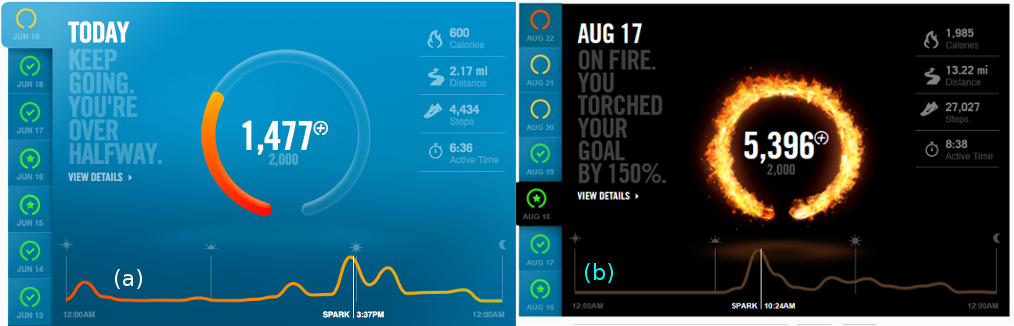
\includegraphics[width=0.9\textwidth]{tworings.png}
		\caption{\footnotesize \textbf{(a):} User halfway to his daily nikefuel goal. \textbf{(b):} User beating his daily limit by 150\% rewarding him with special effects on the ring and a trophy. (Images taken from \cite{fuelbandDcRain} and \cite{fuelbandTechSpce})}.
		\label{fig:tworings}
\end{figure}

The online profile provides detailed information of the users activity, showing steps, calories burned, active time, distance travelled and average fuel. Charts can be displayed for weeks, months or years. This allows the user to track their progress and look at how often they achieve or exceed their goals.\cite{fuelbandTechSpce}.

\begin{figure}[h!]
	\centering
		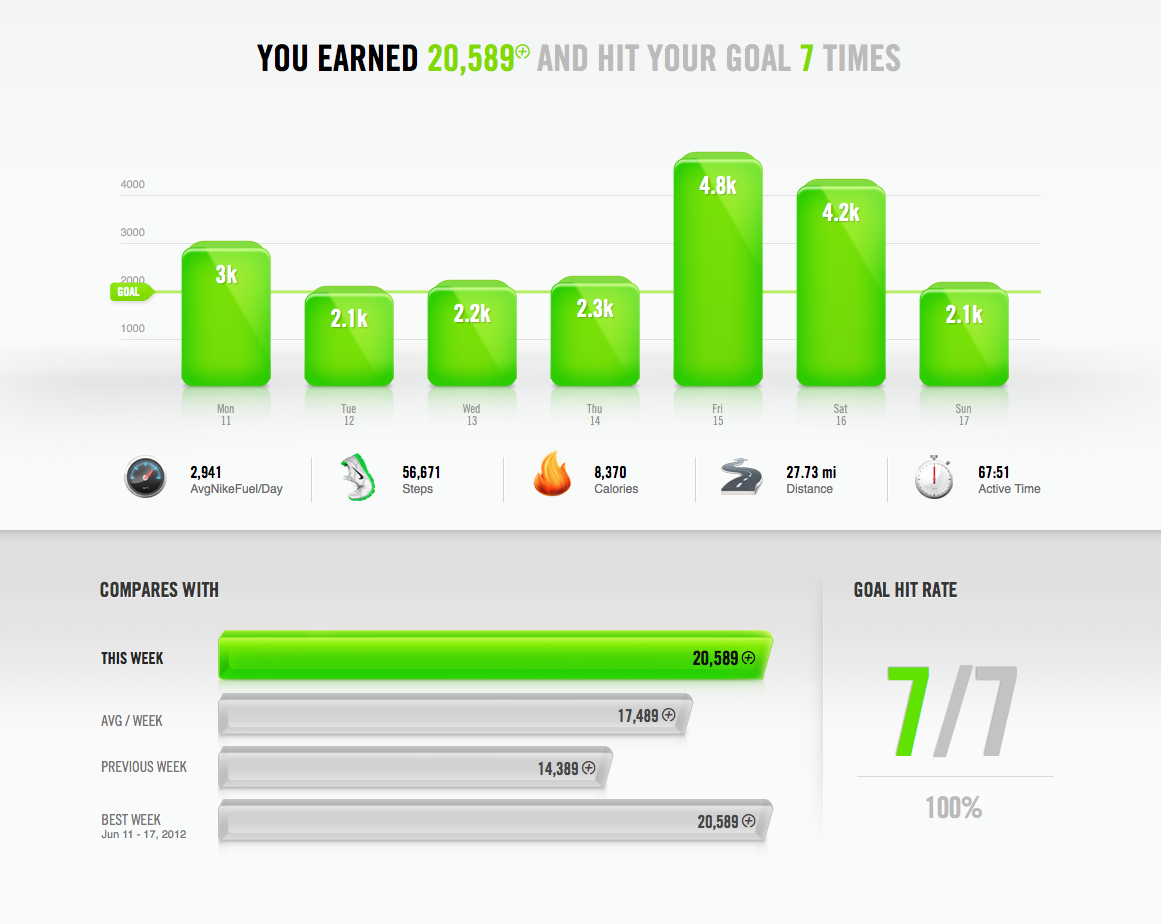
\includegraphics[width=0.7\textwidth]{week.png}
		\caption{\footnotesize The weekly breakdown visulizations presented by Nike+ to the user. \cite{fuelbandTechSpce}}
		\label{fig:activityBreakdown}
\end{figure}

Virtual trophies are awarded for various achievements such as gathering an X amount of NikeFuel or beating the set goal by a 100\%. These trophies can then be shared with friends or displayed on the public profile to show off achievements. The FuelBand can display simple information such as how far the user is from his daily goal, steps taken, and calories burned. A review has reported that the NikeFuel concept can almost become an addiction and lead to doing some last minute workouts in order to reach the goal \cite{fuelbandDcRain}.

\subsection{Fitbit}
Similar to the Nike+, Fitbit allows the user to set daily goals, but as the Fitbit does not use the NikeFuel system, it enables the user to set 3 separate goals: steps taken, floors climbed, and calories burned. The Fitbit does provide an active score, but there is no emphasis on it. A daily activity breakdown is provided, this breaks the activity levels for the day into 4 categories: sedentary, lightly active, fairly active, and very active. All the goal histories can be viewed on the online profile and can be categorized into day, week, months and years. The FitBit Premium service allows the user to splice their data much better providing more detailed information and comparisons. 

\begin{figure}[h!]
	\centering
		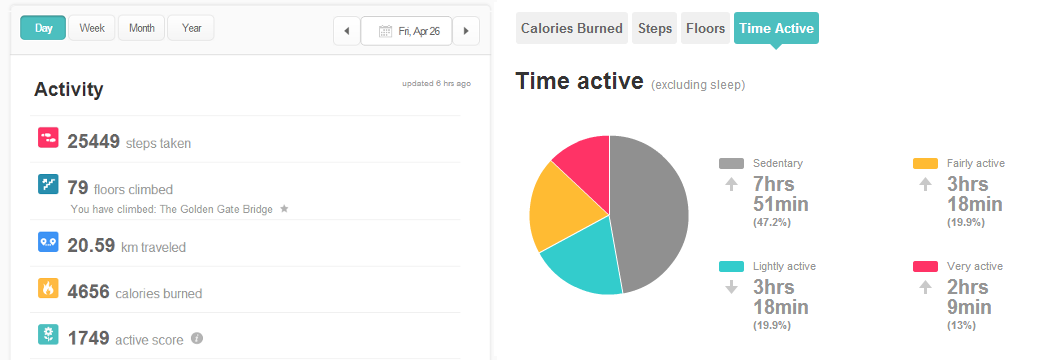
\includegraphics[width=0.9\textwidth]{fitbitActivityBreakdown.png}
		\caption{\footnotesize The breakdown provided by FitBit it can be broken into day, week, month, or year.}
		\label{fig:fitbitActivityBreakdown}
\end{figure}

\subsection{activPal}
Write something around this visulization?

\begin{figure}[h!]
	\centering
		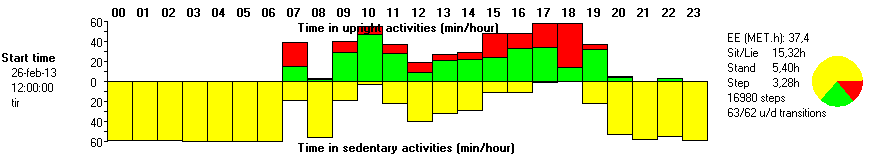
\includegraphics[width=0.9\textwidth]{activPalChart.png}
		\caption{\footnotesize The breakdown provided by FitBit it can be broken into day, week, month, or year.}
		\label{fig:fitbitActivityBreakdown}
\end{figure}

\section{Personal informatics and quantified self}
Currently there are two names that stand out within self-monitoring: Quantified Self, and Personal Informatics. Quantified self is a community of end users who share data and exchange experiences with tools that help them collect information. Personal Informatics on the other hand is academic and developer driven, they desire to understand what makes a good tool, and how the user interacts with such technology.

\subsection{Quantified Self}
In 2011 a movement known as Quantified Self*\cite{quantifiedSelf} had their first conference \cite{bodyHackers}, here people shared data that they had collected about themselves width different types of devices. The goal is to gather as much information about yourself as possible, to learn about yourself through quantitative data. Members of Quantified Self* collect information about everything from sleep patterns and diets to mood and stress levels.

(Cut the next paragraph to shorten this section?)

To promote further development in tools that gather these types of information, the participants of Quantified Self has worked closely with companies and individuals that create personal informatics tools. Devices such as Nike's FuelBand \cite{fuelBand} and Fitbit \cite{fitBit} are results of this cooperation, and both products have been well received.

\subsection{Personal Informatics}
Personal informatics is the label used to classify tools that help people collect personal information for the purpose of self-monitoring and self reflection. These tools are used to help individuals gain self-knowledge about their behaviour, habits, and thoughts\cite{personalInformatics}.

(Cut the next paragraph to shorten the section?)

The Computer-Human Interaction (CHI) conference has since 2010 \cite{chi2010} held workshops and accepted papers on Personal Informatics. The aim is to increase understanding of how the tools affect the user, explore new possibilities, and overall improvement of the user experience.

\section{Medical applications (not a priority)}
Find articles that use body worn sensors for health care